\chapter{Numbers, bits and Boolean algebra}
\label{ch:digital}

Every chapter so far treated voltage as a quantity — 0.227 volts here,
10.45 there. The digital world compresses all of that into two letters:
0 and 1. This chapter introduces the notation (binary, hex, two's
complement), the algebra that manipulates it (truth tables, De Morgan,
Karnaugh maps), and the first sight of a hardware description language —
a 20-line Verilog file that prints gate truth tables. After it, you will
be able to read a byte in any base, prove a simplification two different
ways, and turn an English sentence like ``the alarm sounds when the
ignition is on and the door is open or the belt is off'' into a minimal
gate network.

\section{Why two levels?}
\label{sec:twolevels}

Chapter 6's noise margins are the reason. A ``1'' is not
\qty{3.3}{\volt}; it is \emph{anything above} $V_{IH}$; a ``0'' is
anything below $V_{IL}$. The region between is forbidden — and the
margins $NM_L$, $NM_H$ budget how much noise a signal can pick up before
a receiver misreads it. Two levels, spaced far apart with a guard band,
is the cheapest possible error-correction scheme: any voltage that
drifts stays readable, and every gate regenerates the levels fresh.

\begin{checkpoint}[Two levels, one reason]
Binary is not a mathematical preference — it is the cheapest way to make
physical voltage carry information through noise. Keep asking of every
abstraction above it: \emph{what does a 1 physically mean here?}
\end{checkpoint}

\section{Binary, hex, and two's complement}
\label{sec:repr}

A byte is eight bits, and a number written $b_7b_6\ldots b_0$ means
$\sum_i b_i 2^i$. \emph{Hexadecimal}\index{hexadecimal} groups four bits
per digit (\texttt{0x00}--\texttt{0xFF}); the programmer's muscle memory
is knowing $2^4=16$, $2^8=256$, $2^{10}\approx10^{3}$ cold.

For negatives the convention is \emph{two's
complement}\index{two's complement}: the most significant bit carries
weight $-128$, not $+128$. So \texttt{0xFF} $= -1$, and the representable
range of a signed byte is $-128$ to $+127$ — asymmetric by one. The
payoff: \emph{no subtraction circuit is ever needed}; $a-b$ is just
$a+(\sim b + 1)$, and the same adder does both jobs.

\begin{exercise}[easy]
Write $-1$, $-128$, $+127$ in hex under two's complement; then compute
$100 - 50$ byte-wise without any subtraction: $100 + (\sim50 + 1)$.
\end{exercise}

\section{Truth tables}
\label{sec:tt}

A Boolean function of $n$ inputs has exactly $2^n$ input rows, and its
\emph{truth table}\index{truth table} is the complete enumeration — the
definition, not a summary. Everything later (K-maps, HDL testbenches)
re-arranges or re-prints this table; it is the ground truth.

Here is one in a new notation — \emph{Verilog}\index{Verilog}, the
hardware description language used from chapter 11 onward. You are not
expected to write this yet; read it with the numbered explanations in the
margin of your mind:

\begin{lstlisting}[caption={\ttfamily code/ch08\_gates\_tb.v --- a
behavioral truth printer. Every line explained below the output.},
label={lst:gatestb},abovecaptionskip=0pt]
// ch08_gates_tb.v -- behavioral gate truth printer
`timescale 1ns/1ps
module gates_tb;
  reg  a, b;            // inputs we sweep
  wire y_and, y_or, y_xor, y_nand, y_nor, y_xnor;

  assign y_and  = a & b;
  assign y_or   = a | b;
  assign y_xor  = a ^ b;
  assign y_nand = ~(a & b);
  assign y_nor  = ~(a | b);
  assign y_xnor = ~(a ^ b);

  integer i;
  initial begin
    $display("a b | AND OR XOR NAND NOR XNOR");
    $display("----+---------------------------------");
    for (i = 0; i < 4; i = i + 1) begin
      {a, b} = i[1:0];            // 00,01,10,11 in binary
      #1;
      $display("%b %b |  %b   %b   %b    %b    %b     %b",
               a, b, y_and, y_or, y_xor, y_nand, y_nor, y_xnor);
    end
    $finish;
  end
endmodule
\end{lstlisting}

\begin{lstlisting}[caption={Real output of
\texttt{iverilog -o gates\_tb ch08\_gates\_tb.v \&\& vvp gates\_tb}},
abovecaptionskip=0pt]
a b | AND OR XOR NAND NOR XNOR
----+---------------------------------
0 0 |  0   0   0    1    1     1
0 1 |  0   1   1    1    0     0
1 0 |  0   1   1    1    0     0
1 1 |  1   1   0    0    0     1
ch08_gates_tb.v:28: $finish called at 4000 (1ps)
\end{lstlisting}

Reading the file: \texttt{module}/\texttt{endmodule} wrap a circuit block;
\texttt{reg} holds values we set procedurally, \texttt{wire} is driven
continuously. \texttt{assign} makes a wire follow an expression
forever — that is the hardware, six gates drawn in text.
\texttt{initial ... begin ... end} runs once at simulation start (a
testbench block, not synthesizable). \texttt{\{a,b\}=i[1:0]} splits the
2-bit counter across two wires; \texttt{\#1} waits one tick;
\texttt{\$display} prints. The loop emits all $2^2=4$ rows — the truth
table, printed by the gates themselves.

The symbols for these gates are in Figure~\ref{fig:symbols}; the truth
table above is what each symbol means.

\begin{figure}[htbp]
\centering
% Gate symbols table (circuitikz logic ports, book palette)
\newcommand{\gatesym}[2]{%
  \begin{circuitikz}[baseline=(g.center), scale=0.75, transform shape]
    \node[#1] (g) {};
  \end{circuitikz} & #2 \\}
\begin{tabular}{@{}c l c l@{}}
AND ($ab$)   & \gatesym{american and port}{$y = a\cdot b$} &
NAND ($\overline{ab}$) & \gatesym{american nand port}{$y=\overline{a\cdot b}$} \\
OR ($a+b$)   & \gatesym{american or port}{$y = a+b$} &
NOR ($\overline{a+b}$) & \gatesym{american nor port}{$y=\overline{a+b}$} \\
XOR ($a\oplus b$) & \gatesym{american xor port}{$y = a\oplus b$} &
XNOR ($\overline{a\oplus b}$) & \gatesym{american xnor port}{$y=\overline{a\oplus b}$} \\
NOT ($\bar a$) & \gatesym{american not port}{$y=\bar a$} &
buffer & \gatesym{american buffer port}{$y=a$} \\
\end{tabular}

\caption{The seven gate symbols. Notice the small bubble on NAND, NOR,
XNOR, NOT: an output circle always means ``invert the plain version'' —
$\overline{AND}=NAND$, and so on.}
\label{fig:symbols}
\end{figure}

\begin{exercise}[medium]
From the printed table, write the Boolean expression for XNOR as a sum
of products of $a$, $b$, and their complements.
\end{exercise}

\section{De Morgan and the universal gates}
\label{sec:demorgan}

\begin{definition}[De Morgan's laws]
\index{De Morgan's laws}
\[
\overline{a\cdot b}=\bar a+\bar b,
\qquad
\overline{a+b}=\bar a\cdot\bar b.
\]
NOT distributes by \emph{swapping the operator}. Both directions are
provable by exhaustion — a truth table settles them in four rows.
\end{definition}

The payoff is practical: NAND alone can build every other gate
(Figure~\ref{fig:universal}), and so can NOR — either is a
\emph{universal gate}\index{universal gate}. Real silicon is made of
NANDs; De Morgan is why a designer can sketch in AND/OR and let the
synthesizer retarget to NAND/NOR without changing the function.

\begin{figure}[htbp]
\centering
% NAND universality: NOT, AND, OR from NANDs only
\begin{circuitikz}[american, scale=0.8, transform shape, font=\small]
% NOT from NAND (tie inputs)
\node[american nand port] (n1) at (0,0) {};
\draw (n1.in 1) -- (n1.in 2) to[short,-o] ++(-0.7,0) node[left] {$a$};
\draw (n1.out) to[short,-o] ++(0.4,0) node[right] {$\bar a$};
\node at (0,-1.4) {NOT};
% AND from NAND + NAND-NOT
\node[american nand port] (n2) at (3.4,0) {};
\node[american nand port] (n3) at (5.4,0) {};
\draw (n2.in 1) to[short,-o] ++(-0.7,0) node[left] {$a$};
\draw (n2.in 2) to[short,-o] ++(-0.7,0) node[left] {$b$};
\draw (n3.in 1) -- (n3.in 2);
\draw (n2.out) -- ++(0.6,0) |- (n3.in 1) -- ++(-0.6,0);
\draw (n3.out) to[short,-o] ++(0.4,0) node[right] {$ab$};
\node at (4.4,-1.4) {AND};
% OR from NAND-NOT inputs + NAND
\node[american nand port] (n4) at (8.0,0.5) {};
\node[american nand port] (n5) at (8.0,-0.9) {};
\node[american nand port] (n6) at (10.2,-0.2) {};
\draw (n4.in 1) -- (n4.in 2) to[short,-o] ++(-0.7,0) node[left] {$a$};
\draw (n5.in 1) -- (n5.in 2) to[short,-o] ++(-0.7,0) node[left] {$b$};
\draw (n4.out) -| (n6.in 1);
\draw (n5.out) -| (n6.in 2);
\draw (n6.out) to[short,-o] ++(0.4,0) node[right] {$a+b$};
\node at (9.0,-2.0) {OR (De Morgan)};
\end{circuitikz}

\caption{NAND building NOT, AND, and OR. Notice the OR shape: two
NAND-inverters feeding a NAND — that is De Morgan drawn in wires.}
\label{fig:universal}
\end{figure}

\begin{exercise}[medium]
Draw NOT, AND, and OR out of NOR gates only. (Hint: NOT is one NOR;
work through De Morgan.)
\end{exercise}

\section{Worked example 1: signed byte arithmetic, three ways}
\label{sec:we-bytes}

\textbf{Strategy.} Compute $45 - 83$ in an 8-bit byte three different
ways and watch them land on the same answer — that agreement is what
makes two's complement worth its asymmetry.

\textbf{Solution.}
\begin{enumerate}
\item \emph{Plain arithmetic}: $45-83=-38$. In signed hex,
$-38 = 256-38 = 218 = \texttt{0xDA}$.
\item \emph{Negate and add}: $-83$ is $\sim83+1 = \sim\texttt{0x53}+1 =
\texttt{0xAC}+1=\texttt{0xAD}$. Then $45+\texttt{0xAD} =
\texttt{0x2D}+\texttt{0xAD} = \texttt{0xDA}$ — the carry out of bit 7 is
discarded; the byte wraps and the answer is right.
\item \emph{Bit-check}: \texttt{0xDA} $=1101\,1010_2$: top bit $-128$ plus
$64+16+8+2=90$, total $-128+90=-38$. \checkmark
\end{enumerate}

The same adder did the subtraction; method 2 is literally what silicon
computes.

\section{Worked example 2: prove a simplification twice}
\label{sec:we-simp}

\textbf{Strategy.} Take $y = ab + a\bar b + \bar a b$. Prove it equals
$a+b$ first by exhaustion (truth table) then by algebra — the two proofs
compliment each other: the table is infallible but proves only this
instance; the algebra shows \emph{why} and generalizes.

\textbf{Solution.}
\begin{lstlisting}[caption={Truth-table check via
\texttt{ch08\_truth\_check.py} --- all 4 rows agree.},abovecaptionskip=0pt]
vars: A B
A B | A&B | A&~B | ~A&B   A|B
-----------------------------
0 0 |   0   0
0 1 |   1   1
1 0 |   1   1
1 1 |   1   1
EQUIVALENT on all 4 input rows
\end{lstlisting}

Algebraically: $ab + a\bar b = a(b+\bar b) = a$, so $y = a + \bar a b =
a + b$ (using $x + \bar x y = x + y$). Same conclusion, one line.

The checker used above is the book's truth-table tool — exercises will
meet it again:

\begin{lstlisting}[caption={\ttfamily code/ch08\_truth\_check.py ---
compares expressions exhaustively and prints every row.},
label={lst:tcheck},abovecaptionskip=0pt]
usage: python3 ch08_truth_check.py "I&D | I&~B" "I&(D|~B)"
# evaluates each expression on all 2^n input rows, prints the table,
# then EQUIVALENT or DIFFERENT with the first counterexample.
\end{lstlisting}

\section{Worked example 3: the alarm circuit}
\label{sec:we-alarm}

\textbf{Strategy.} ``The alarm buzzes when the ignition is on and either
the door is open or the seatbelt is unfastened.'' Name the inputs
$I, D, B$ (belt fastened = 1), write the truth table, reduce with a
K-map, then build three equivalent gate networks.

\textbf{Solution.} Rows where the alarm is off ($I=0$) are all zero;
when $I=1$, the alarm sounds for $D=1$ or $B=0$. The 3-variable K-map
(Figure~\ref{fig:kmap3}) groups two overlapping pairs:
$I\bar B$ and $ID$, giving
\[
y = I\cdot D + I\cdot\bar B = I\,(D+\bar B).
\]

\begin{lstlisting}[caption={Checker confirms the factored form
(verbatim).},abovecaptionskip=0pt]
vars: B D I
B D I | I&D | I&~B   I&(D|~B)
-----------------------------
0 0 0 |   0   0
0 0 1 |   1   1
0 1 0 |   0   0
0 1 1 |   1   1
1 0 0 |   0   0
1 0 1 |   0   0
1 1 0 |   0   0
1 1 1 |   1   1
EQUIVALENT on all 8 input rows
\end{lstlisting}

\begin{figure}[htbp]
\centering
% 3-var K-map for the alarm: I&D | I&~B -> I&D + I&~B
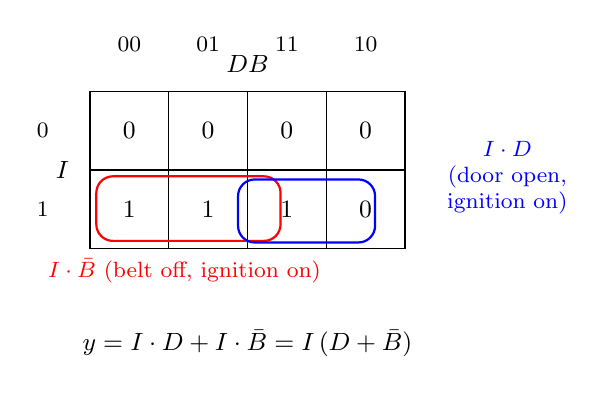
\begin{tikzpicture}[font=\small]
\draw[step=1] (0,0) grid (4,2);
\node at (-0.35,1.0) {$I$}; \node at (2.0,2.35) {$DB$};
\node[font=\footnotesize] at (-0.6,1.5) {0}; \node[font=\footnotesize] at (-0.6,0.5) {1};
\node[font=\footnotesize] at (0.5,2.6) {00}; \node[font=\footnotesize] at (1.5,2.6) {01};
\node[font=\footnotesize] at (2.5,2.6) {11}; \node[font=\footnotesize] at (3.5,2.6) {10};
% I row (bottom, I=1): DB cols 00->1, 01->1, 11->1, 10->0
\node at (0.5,0.5) {1}; \node at (1.5,0.5) {1}; \node at (2.5,0.5) {1}; \node at (3.5,0.5) {0};
\node at (0.5,1.5) {0}; \node at (1.5,1.5) {0}; \node at (2.5,1.5) {0}; \node at (3.5,1.5) {0};
\draw[red, thick, rounded corners=6pt] (0.08,0.10) rectangle (2.42,0.92);
\node[red, font=\footnotesize] at (1.2,-0.28) {$I\cdot\bar B$ (belt off, ignition on)};
\draw[blue, thick, rounded corners=6pt] (1.88,0.08) rectangle (3.62,0.88);
\node[blue, font=\footnotesize, align=center] at (5.3,0.9) {$I\cdot D$\\ (door open,\\ ignition on)};
\node at (2.0,-1.2) {$y = I\cdot D + I\cdot\bar B = I\,(D+\bar B)$};
\end{tikzpicture}

\caption{The alarm's 3-variable K-map. Notice the wrap: the $DB$ columns
run 00, 01, 11, 10 — a Gray-code order, so adjacent cells always differ
by exactly one bit; that is what makes groupings meaningful.}
\label{fig:kmap3}
\end{figure}

\begin{figure}[htbp]
\centering
% same function three ways: SOP AND-OR, factored, NAND-only
\begin{circuitikz}[american, scale=0.72, transform shape, font=\footnotesize]
% --- 1) AND-OR SOP: I&D + I&~B ---
\node[american not port] (nB) at (0.6,1.9) {};
\draw (nB.in) to[short,-o] ++(-0.5,0) node[left] {$B$};
\node[american and port] (a1) at (2.2,2.0) {};
\node[american and port] (a2) at (2.2,0.4) {};
\node[american or port] (o1) at (4.4,1.2) {};
\draw (nB.out) -| (a1.in 1);
\draw (a1.in 2) to[short,-o] ++(-1.9,0) node[left] {$I$};
\draw (a2.in 1) to[short,-o] ++(-1.9,0) node[left] {$I$};
\draw (a2.in 2) to[short,-o] ++(-1.9,0) node[left] {$D$};
\draw (a1.out) -| (o1.in 1); \draw (a2.out) -| (o1.in 2);
\draw (o1.out) to[short,-o] ++(0.5,0) node[right] {$y$};
\node at (2.6,-0.7) {$I\bar B + ID$};
% --- 2) factored: I(D + ~B) ---
\begin{scope}[xshift=7.2cm]
\node[american not port] (nB2) at (0.6,1.9) {};
\draw (nB2.in) to[short,-o] ++(-0.5,0) node[left] {$B$};
\node[american or port] (o2) at (2.2,1.2) {};
\node[american and port] (a3) at (4.4,0.9) {};
\draw (nB2.out) -| (o2.in 1);
\draw (o2.in 2) to[short,-o] ++(-1.9,0) node[left] {$D$};
\draw (a3.in 1) to[short,-o] ++(-0.9,0) node[left] {$I$};
\draw (o2.out) -| (a3.in 2);
\draw (a3.out) to[short,-o] ++(0.5,0) node[right] {$y$};
\node at (2.6,-0.7) {$I(D+\bar B)$};
\end{scope}
\end{circuitikz}
\vspace{4pt}
\begin{circuitikz}[american, scale=0.72, transform shape, font=\footnotesize]
% --- 3) NAND-only: ~( ~(I~B) * ~(ID) ) = (IB')' (ID)' then NAND them ---
\node[american not port] (nB3) at (0.6,1.9) {};
\draw (nB3.in) to[short,-o] ++(-0.5,0) node[left] {$B$};
\node[american nand port] (na) at (2.6,2.0) {};
\node[american nand port] (nb) at (2.6,0.4) {};
\node[american nand port] (nc) at (4.8,1.2) {};
\draw (nB3.out) -| (na.in 1);
\draw (na.in 2) to[short,-o] ++(-2.3,0) node[left] {$I$};
\draw (nb.in 1) to[short,-o] ++(-2.3,0) node[left] {$I$};
\draw (nb.in 2) to[short,-o] ++(-2.3,0) node[left] {$D$};
\draw (na.out) -| (nc.in 1); \draw (nb.out) -| (nc.in 2);
\draw (nc.out) to[short,-o] ++(0.5,0) node[right] {$y$};
\node at (2.8,-0.8) {NAND-only: $(I\bar B)' \cdot (ID)'$ NANDed};
\end{circuitikz}

\caption{The same alarm function three ways: sum-of-products, factored,
and NAND-only. The NAND version costs one more gate but uses a single
gate type — the trade real fabs make everywhere.}
\label{fig:threeways}
\end{figure}

\begin{exercise}[hard]
(Implement) The minimal form is $I\,(D+\bar B)$. Use the checker on
your machine to prove the sum-of-products and NAND-only forms agree on
all 8 rows; then decide which a fab would rather print.
\end{exercise}

\section{From expression to network}
\label{sec:pipeline}

The workflow this chapter just walked is a pipeline
(Figure~\ref{fig:pipeline}): sentence $\to$ truth table $\to$ K-map
$\to$ minimal sum-of-products $\to$ gate network. The same reduction a
synthesizer does in nanoseconds — learning to do it by hand is how you
\emph{audit} what the tool did, and why HDLBits drills (named in the
exercises) start at truth tables.

\begin{figure}[htbp]
\centering
% truth table -> K-map -> minimal expression pipeline
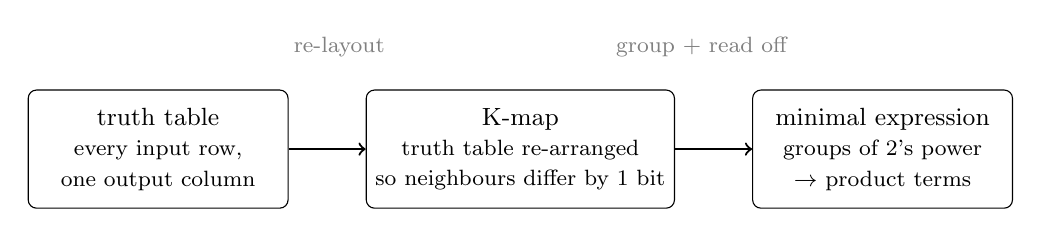
\begin{tikzpicture}[font=\small, box/.style={draw, rounded corners=3pt, align=center, minimum height=1.5cm, minimum width=3.3cm}]
\node[box] (tt) at (0,0) {truth table\\ \footnotesize every input row,\\ \footnotesize one output column};
\node[box] (km) at (4.6,0) {K-map\\ \footnotesize truth table re-arranged\\ \footnotesize so neighbours differ by 1 bit};
\node[box] (ex) at (9.2,0) {minimal expression\\ \footnotesize groups of 2's power\\ \footnotesize $\to$ product terms};
\draw[->, thick] (tt) -- (km);
\draw[->, thick] (km) -- (ex);
\node[font=\footnotesize, text=gray] at (2.3,1.3) {re-layout};
\node[font=\footnotesize, text=gray] at (6.9,1.3) {group + read off};
\end{tikzpicture}

\caption{The minimization pipeline. Notice which step is mechanical
(K-map re-layout is just a permutation of the truth table's rows) and
which step carries judgment (choosing the groups).}
\label{fig:pipeline}
\end{figure}

The 2-variable map of Figure~\ref{fig:kmap2} is the same picture,
smaller — the groups it draws are the exact terms of Worked Example 2.

\begin{figure}[htbp]
\centering
% 2-var K-map for AB + A~B + ~AB = A + B
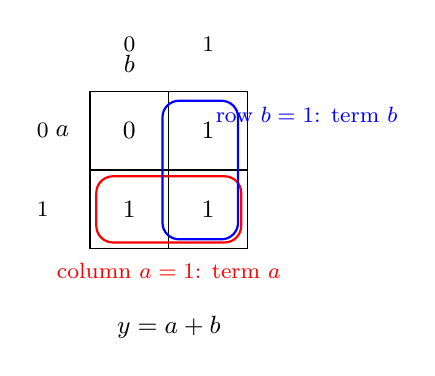
\begin{tikzpicture}[font=\small]
\draw[step=1] (0,0) grid (2,2);
\node at (-0.35,1.5) {$a$}; \node at (0.5,2.35) {$b$};
\node[font=\footnotesize] at (-0.6,1.5) {0}; \node[font=\footnotesize] at (-0.6,0.5) {1};
\node[font=\footnotesize] at (0.5,2.6) {0}; \node[font=\footnotesize] at (1.5,2.6) {1};
\node at (0.5,1.5) {0}; \node at (1.5,1.5) {1};
\node at (0.5,0.5) {1}; \node at (1.5,0.5) {1};
\draw[red, thick, rounded corners=6pt] (0.08,0.08) rectangle (1.92,0.92);
\node[red, font=\footnotesize] at (1.0,-0.28) {column $a=1$: term $a$};
\draw[blue, thick, rounded corners=6pt] (0.92,0.12) rectangle (1.88,1.88);
\node[blue, font=\footnotesize] at (2.75,1.7) {row $b=1$: term $b$};
\node at (1.0,-1.0) {$y = a + b$};
\end{tikzpicture}

\caption{The 2-variable K-map for $ab+a\bar b+\bar ab$: two groups of two
read off $a$ and $b$ directly.}
\label{fig:kmap2}
\end{figure}

\section{Common mistakes}
\label{sec:mistakes08}

\begin{itemize}
\item \textbf{Misreading place values} on multi-digit binary: read the
exponents, don't count digits — $10_2$ is two, not ten; \texttt{0x10} is
sixteen, not ``one-zero''.
\item \textbf{Sign slips in two's complement}: forgetting the top bit is
$-2^{n-1}$ gives wrong negatives; $\sim x$ alone is $-x-1$, not $-x$.
\item \textbf{Off-by-one on representable ranges}: a signed byte is
$-128\ldots+127$, asymmetric — you cannot negate $-128$ in 8 bits.
\item \textbf{Applying De Morgan halfway}: $\overline{ab}\ne\bar a\bar b$
— the operator must swap too.
\item \textbf{Thinking K-map adjacency is physical adjacency}: edges wrap
(left-right, top-bottom) because it's a torus, not a table.
\end{itemize}

\section{Exercises}
\label{sec:exercises08}

\begin{exercise}[easy]
Convert \texttt{0b10110010} to hex and decimal (unsigned) and to decimal
(signed).
\end{exercise}
\begin{exercise}[easy]
What is $-1 - 1$ in an 8-bit two's-complement byte? Show the hex.
\end{exercise}
\begin{exercise}[easy]
Write the truth table of $y=\bar a\bar b+\bar a b$. What common gate is it?
\end{exercise}
\begin{exercise}[easy]
Prove $\overline{a+b}=\bar a\bar b$ by exhaustion on all four input rows.
\end{exercise}
\begin{exercise}[medium]
Transform $\overline{\bar a + bc}$ into a product form without any
complement-of-a-sum remaining.
\end{exercise}
\begin{exercise}[medium]
Minimize $y = \bar a\bar b + a\bar b + ab$ and state the gate count
before and after.
\end{exercise}
\begin{exercise}[medium]
On paper, derive the alarm minimal form a second way: from the truth
table, write the full sum-of-products, then factor and absorb without a
K-map.
\end{exercise}
\begin{exercise}[medium]
In 8-bit two's complement, what is \texttt{0x7F + 1}? Name the
phenomenon.
\end{exercise}
\begin{exercise}[hard]
Design: a hallway light is on when (motion) or (dark and switch-on).
Derive minimal SOP from a truth table, then implement the truth
equivalence check in \texttt{ch08\_truth\_check.py} on the two forms.
Then do HDLBits ``Getting Started'' + the basic-gates set as external
drills.
\end{exercise}
\begin{exercise}[hard]
Prove XOR is also universal: build NOT, AND, OR from XOR + constants +
wires, or argue which one fails and why (this is a trick — one of them
cannot be built; identify which and say why).
\end{exercise}

\section{Summary}
\label{sec:summary08}

\begin{center}\small
\begin{tabular}{@{}p{0.32\linewidth}p{0.60\linewidth}@{}}
\toprule
\textbf{Idea} & \textbf{One-line version} \\ \midrule
Two levels & Cheapest noise immunity: wide rails + guard band. \\
Binary / hex & Place value $2^i$; hex = 4-bit shorthand. \\
Two's complement & Top bit weighs $-2^{n-1}$; adder subtracts free. \\
Truth table & The definition; $2^n$ rows is the whole function. \\
De Morgan & NOT distributes by swapping AND$\leftrightarrow$OR. \\
Universal gates & NAND alone, or NOR alone, builds everything. \\
K-map & Truth table re-laid so neighbours differ by one bit; groups of 2's power read off minimal SOP. \\
Synthesis & The pipeline sentence$\to$table$\to$map$\to$gates is what the tools automate. \\
\bottomrule
\end{tabular}
\end{center}

\section*{Notes}
\begin{enumerate}
\item \emph{All About Circuits}, Vol.~IV: Digital, ch.\ 1--8 — numerals,
Boolean algebra, gate properties, De Morgan, Karnaugh
maps~\cite{aacvol4}.
\item Harris \& Harris, \emph{Digital Design and Computer Architecture},
ch.\ 1--2 — chapter ordering and exercise style adapted
here~\cite{ddca}.
\end{enumerate}

\section*{Hints and answers}
\begin{description}
\item[Byte sign (easy)] \texttt{0xFF}=$-1$, \texttt{0x80}=$-128$,
\texttt{0x7F}=$+127$; $100+(\sim50+1)=100+206=306\to306-256=50$.
\item[XNOR SOP (medium)] $\bar a\bar b + ab$.
\item[NOR-only (medium)] NOT: tie inputs ($\overline{a+a}=\bar a$);
OR: one NOR ($\overline{a+b}$) inverted by NOR-NOT; AND: invert each
input with NOR-NOT, then NOR.
\item[Hex-dec (easy)] \texttt{0b10110010}=\texttt{0xB2}=178 unsigned,
$-78$ signed.
\item[Wrap (easy)] \texttt{0xFE}=$-2$.
\item[Gate ID (easy)] $\bar a$.
\item[De Morgan (easy)] Rows $00{:}1{=}1$; $01{:}0{=}0$; $10{:}0{=}0$;
$11{:}0{=}0$.
\item[Transform (medium)] $a\cdot\overline{bc}=a(\bar b+\bar c)$.
\item[Minimize (medium)] $y=\bar b+ab$ $\to$ then $\bar b+a$: 4 gates
$\to$ 1 (using $x+\bar xy=x+y$).
\item[Alarm, algebraic (medium)] $ID+I\bar B=I(D+\bar B)$ directly from
factoring; SOP full form collects the same three minterms.
\item[Overflow (medium)] \texttt{0x80} — signed overflow from $+127$ to
$-128$.
\item[Hallway (hard)] $y=M+DS$; verify both forms equivalent on all 8
rows; HDLBits drills build the same muscle in real HDL.
\item[XOR trick (hard)] AND cannot be built: XOR is affine —
every output is an XOR of inputs and constants, and AND is not affine.
\end{description}
